\documentclass[../main.tex]{subfiles}
\begin{document}
\chapter{The Double-$\tau_h$ + jet trigger}

In view of Run 3, a lot of effort has been dedicated in order to maximize the collection efficiency from physics processes with much smaller cross sections than the backgrounds, as is the case for both $H\to\tau\tau$ and $HH\to bb\tau\tau$ processes. In these two cases, in most events the produced $\tau\tau$ pair is accompanied by one or more jets coming from the hard-scattering processes or from QCD radiation (in addition to the 2 $b$-jets coming from the other $H$ in the $HH\to bb\tau\tau$ process), as seen in Fig.~\ref{hh:fig:trig_ngenjets}. 


Therefore, by requiring at trigger level an additional jet (whose $p_t$ spectre is shown in Fig.~\ref{hh:fig:trig_l1jet_pt}) on top of the already present double-$\tau_h$ trigger, the $p_t$ threshold on the $\tau_h$ could be lowered. By doing so, as more $\tau_h$ will be available for triggering (see Fig.~\ref{hh:fig:trig_l1tau_pt}), the acceptance of both analysis could be enlarged.


\begin{figure}[h!]
\begin{center}
\subfloat{\includegraphics[width=0.5\textwidth]{Images/ngenjet_htt_ggf}}
\subfloat{\includegraphics[width=0.5\textwidth]{Images/ngenjet_hhbbtt_ggf}}
\end{center}
\caption{Number of jets  per event at generator level for $H\to\tau\tau$ ggH (left) and $HH\to bb\tau\tau$ ggHH (right) processes.}
\label{hh:fig:trig_ngenjets}
\end{figure}

\begin{figure}[h!]
\begin{center}
\subfloat{\includegraphics[width=0.5\textwidth]{Images/leading_jet_pt_htt_ggf}}
\subfloat{\includegraphics[width=0.5\textwidth]{Images/leading_jet_pt_hhbbtt_ggf}}
\end{center}
\caption{L1 leading jet $p_t$ for the $H\to\tau\tau$ ggH (left) and $HH\to bb\tau\tau$ ggHH (right) processes.}
\label{hh:fig:trig_l1jet_pt}
\end{figure}

\begin{figure}[h!]
\begin{center}
\subfloat{\includegraphics[width=0.5\textwidth]{Images/l1tau_pt_htt_ggf}}
\subfloat{\includegraphics[width=0.5\textwidth]{Images/l1tau_pt_hhbbtt_ggf}}
\end{center}
\caption{L1 leading and subleading $\tau_h$ $p_t$ for the $H\to\tau\tau$ ggH (left) and $HH\to bb\tau\tau$ ggHH (right) processes.}
\label{hh:fig:trig_l1tau_pt}
\end{figure}

In the following sections we will discuss the design and performance of a new seed with two $\tau_h$ and one jet to be included in the L1 Menu and a new HLT path seeded by this new L1 seed. The figures of merit of these new seed and path will be adding as low rate as possible but increasing the final acceptance on the $H\to\tau\tau$ and $HH\to bb\tau\tau$ analysis. This acceptance will come not only from the new trigger, but also from the offline selections applied. In the $H\to\tau\tau$ analysis \cite{hh:htt_run2}, the two $\tau_h$ are selected if their $p_T > 40$~GeV, while the selection on the jets varies depending on the category considered among four different categories. In the following study we will consider two categories, obtained as a simplification of the analysis categories: the 1-jet, high $p_t$ category, where we consider events with one jet with $p_T > 70$~GeV, and the 2-jet category, where we ask for two jets with $p_T > 30$~GeV. In the $HH\to bb\tau\tau$, as was described in Chapter~\ref{hh:chapter:analysis}, the two $\tau_h$ are selected among the ones with $p_t>40$~GeV, while the jet candidates must have a $p_t>20$~GeV.



\section{The L1 Double-$\tau_h$ + jet trigger}
\label{hh:sec:l1seeds}

In the L1 menu used during the Run-2 taking, the only seeds that consider $\tau_h$ were the \texttt{L1\_DoubleIsoTauXer2p1} seeds, where two isolated $\tau_h$ with $p_t\geq X$~GeV and $|\eta|<2.1$ are selected. The threshold $X$ varied during the data-taking, taking a value $X=32~$GeV during 2018. The strategy we will follow in this study is to include a new seed in the L1 Menu with two isolated $\tau_h$ objects and one jet object identified by the $\mu$GT. This way, it could complement the already present double-$\tau_h$ seed with the same 32~GeV threshold or with a bigger $p_t$ threshold in order to keep the rate as low as possible. However, a particular treatment has to be given to seeds involving $\tau_h$ and jet objects simultaneously, as both are reconstructed as purely calorimetric objects. Then, all $\tau_h$ objects will enter the L1 jet collection, while some of the L1 jets will also appear in the L1 $\tau_h$ collection. This issue can be perfectly seen in Fig.~\ref{hh:fig:l1_tau_jet_dR}. To reduce this effect, a feature called overlap removal \cite{intro:l1_13tev} is used, so only L1 jets that are separated more than $\Delta R>0.5$ with the selected $\tau_h$ are considered. This feature was present in the $\mu$GT before the inclusion of the seeds, although none of the already present seeds were using it and, in fact, it had to be tuned before attempting the inclusion of the new seeds.

\begin{figure}[h!]
\begin{center}
\includegraphics[width=0.5\textwidth]{Images/l1_tau_jet_dR}
\end{center}
\caption{Minimal $\Delta R$ between all L1 $\tau_h$'s and jets per event in a $H\to\tau\tau$ ggH simulated sample. The peak appearing at small $\Delta R$ values is due to the overlap between the L1 $\tau_h$ and jet collections.}
\label{hh:fig:l1_tau_jet_dR}
\end{figure}

As previously stated, this new double-$\tau_h$+jet seed (encoded as \texttt{L1\_Double\-IsoTauY\-er2p1\-\_JetZ\_RmOvlp\_dR0p5}) does not aim to replace the present \texttt{L1\_Double\-Iso\-Tau32er2p1} seed, but to complement it. However, increasing the double-$\tau_h$ $p_t$ threshold to a value $X$ could be needed in order to make some rate available to the new seed. The rates corresponding to different values of the double-$\tau_h$ threshold are shown in Fig.~\ref{hh:fig:trig_ditau32_rate}. These rates are estimated using a zero bias data sample taken during a 2018 run but with Run-3 conditions applied (PU linearly scaled to 53 and 2748 colliding bunches). After the inclusion of the new seed, the aim is to keep the rate as close as possible to the rate coming from the \texttt{L1\_Double\-Iso\-Tau32er2p1} seed, so a target rate of $\sim17$~kHz will be considered.

\begin{figure}[h!]
\begin{center}
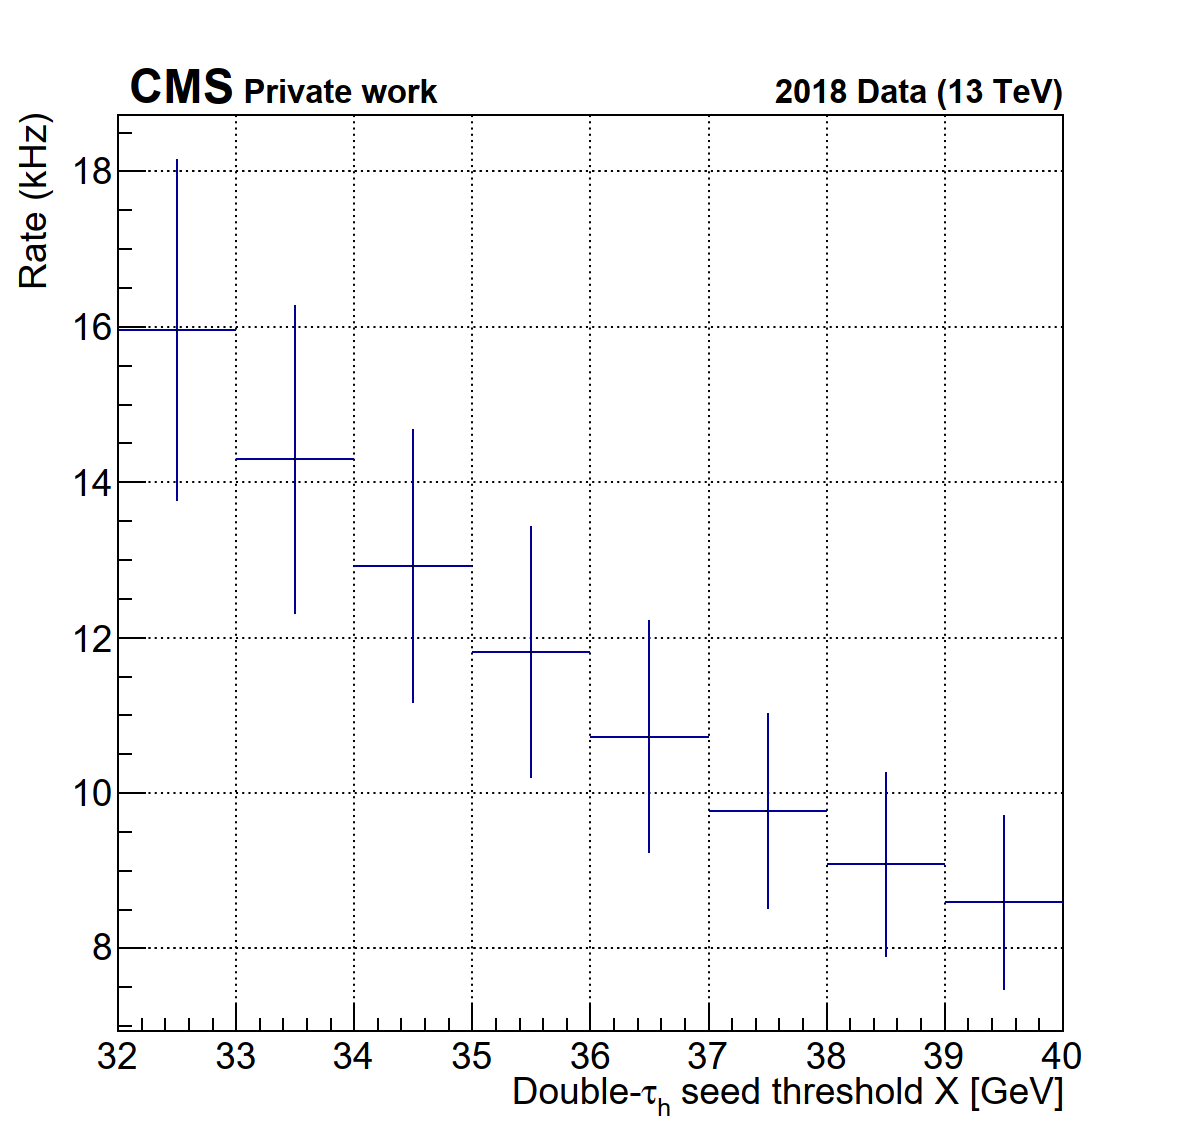
\includegraphics[width=0.5\textwidth]{Images/plot2D_ditau_sym_323755}
\end{center}
\caption{Rate of the \texttt{L1\_DoubleIsoTauXer2p1} trigger seed as a function of the $X$ threshold.}
\label{hh:fig:trig_ditau32_rate}
\end{figure}

As we would like to increase the signal acceptance, we will compute the acceptance gain when considering the two new seeds instead of the reference \texttt{L1\_Double\-IsoTau32\-er2p1} seed. In this case we will consider four signal samples, two ggH and VBFH $H\to\tau\tau$ and two ggHH and VBFHH $HH\to bb\tau\tau$. These acceptance gains are computed not only asking that the L1 objects pass the required selection cuts (grouped in the booleans \texttt{PassL1DoubleTau32}, \texttt{PassL1DoubleTauX} and \texttt{PassL1DoubleTauYJetZ}), but also applying selections to the objects obtained by the offline reconstruction system that evolve accordingly to the L1 thresholds considered. In general, this evolution means that, for a given L1 $p_t$ threshold $T$, the offline threshold is obtained as $T$ + $\Delta T$. As in both target analysis the offline threshold is set to 40~GeV when using a L1 threshold of 32~GeV, we will consider $\Delta T=8$~GeV for the $\tau_h$. For the jets we will consider $\Delta T=10$~GeV. All $p_t$ selections are summarised in Table~\ref{hh:tab:trig_offpt}, where one boolean associated to each seed has been defined to group the needed selections. On top of these $p_t$ cuts, we ask all offline jets to have $|\eta|<4.7$ and pass tight jet ID and loose PU jet ID and an overlap removal criteria with the offline $\tau_h$.

\begin{table}
	\begin{center}
	\begin{tabular}{c || c | c | c }
		                           & \multicolumn{3}{c}{Offline $p_t$ selections} \\
		Boolean                    & 1-jet, high $p_t$ & 2-jet & bb$\tau\tau$ \\\hline\hline
		\texttt{PassOfflDoubleTau32} & 
			$\begin{matrix}
				p_t^{\tau_1}>40\\
				p_t^{\tau_2}>40\\
				p_t^{j_1}>70
			\end{matrix}$ &
			$\begin{matrix}
				p_t^{\tau_1}>40\\
				p_t^{\tau_2}>40\\
				p_t^{j_1}>30 \\
				p_t^{j_2}>30
			\end{matrix}$ &
			$\begin{matrix}
				p_t^{\tau_1}>40\\
				p_t^{\tau_2}>40\\
				p_t^{j_1}>20\\
				p_t^{j_2}>20
			\end{matrix}$ \\\hline
		\texttt{PassOfflDoubleTauX} & 
			$\begin{matrix}
				p_t^{\tau_1}>X+8\\
				p_t^{\tau_2}>X+8\\
				p_t^{j_1}>70
			\end{matrix}$ &
			$\begin{matrix}
				p_t^{\tau_1}>X+8\\
				p_t^{\tau_2}>X+8\\
				p_t^{j_1}>30 \\
				p_t^{j_2}>30
			\end{matrix}$ &
			$\begin{matrix}
				p_t^{\tau_1}>X+8\\
				p_t^{\tau_2}>X+8\\
				p_t^{j_1}>20\\
				p_t^{j_2}>20
			\end{matrix}$ \\\hline
		\texttt{PassOfflDoubleTauYJetZ} &
			$\begin{matrix}
				p_t^{\tau_1}>Y+8\\
				p_t^{\tau_2}>Y+8\\
				p_t^{j_1}>Z+10 \\
				p_t^{j_1}>70
			\end{matrix}$ &
			$\begin{matrix}
				p_t^{\tau_1}>Y+8\\
				p_t^{\tau_2}>Y+8\\
				p_t^{j_1}>Z+10 \\
				p_t^{j_1}>30 \\
				p_t^{j_2}>30
			\end{matrix}$ &
			$\begin{matrix}
				p_t^{\tau_1}>Y+8\\
				p_t^{\tau_2}>Y+8\\
				p_t^{j_1}>Z+10 \\
				p_t^{j_1}>20 \\
				p_t^{j_2}>20
			\end{matrix}$
	\end{tabular}
	\end{center}

	\caption{Offline $p_t$ selections associated to the L1 selections of \texttt{L1\_DoubleIsoTau32er2p1}, \texttt{L1\_DoubleIsoTauXer2p1} and \texttt{L1\_DoubleIsoTauYer2p1\_JetZ\_RmOvlp\_dR0p5}, where $\tau_1$ and $\tau_2$ are the leading and subleading $\tau_h$ and $j_1$ and $j_2$ are the leading and subleading jets. All thresholds are expressed in GeV.}
	\label{hh:tab:trig_offpt}
\end{table}


Thus, the acceptance gain when adding a double-$\tau_h$+jet seed and modifying the threshold of the present double-$\tau_h$ seed can be defined as
\begin{equation}
g(X, Y, Z) = \frac{\begin{matrix}N[(\text{\texttt{PassL1DoubleTauX}} \,\,\&\&\,\, \text{\texttt{PassOfflDoubleTauX}}) \,\,||\,\, \\ \qquad\qquad\qquad(\text{\texttt{PassL1DoubleTauYJetZ}} \,\,\&\&\,\, \text{\texttt{PassOfflDoubleTauYJetZ}})] \end{matrix}}{N[\text{\texttt{PassL1DoubleTau32}} \,\,\&\&\,\, \text{\texttt{PassOfflDoubleTau32}}]}
\end{equation}
where $N$ is the number of events that pass the conditions required. The average acceptance gains for the samples and categories considered is shown in Fig.~\ref{hh:fig:l1_trig_mean_acc} (only the 20 sets with the highest acceptance gain in a 15-16 kHz rate range are displayed). Given these results, the decision was to consider thresholds $Y=26$ and $Z=55$ GeV for the double-$\tau_h$+jet seed. However, another double-$\tau_h$+jet seed with thresholds $Y=26$ GeV and $Z=70$ GeV was added as a backup seed in case the rate coming from the main seed ends up being bigger than expected. Rates for these new seeds and their main acceptance gains on top of the \texttt{L1\_DoubleIsoTau32er2p1} seed for the two processes considered are shown in Table~\ref{hh:tab:l1trig:allseeds}.

\begin{figure}
\subfloat{\centering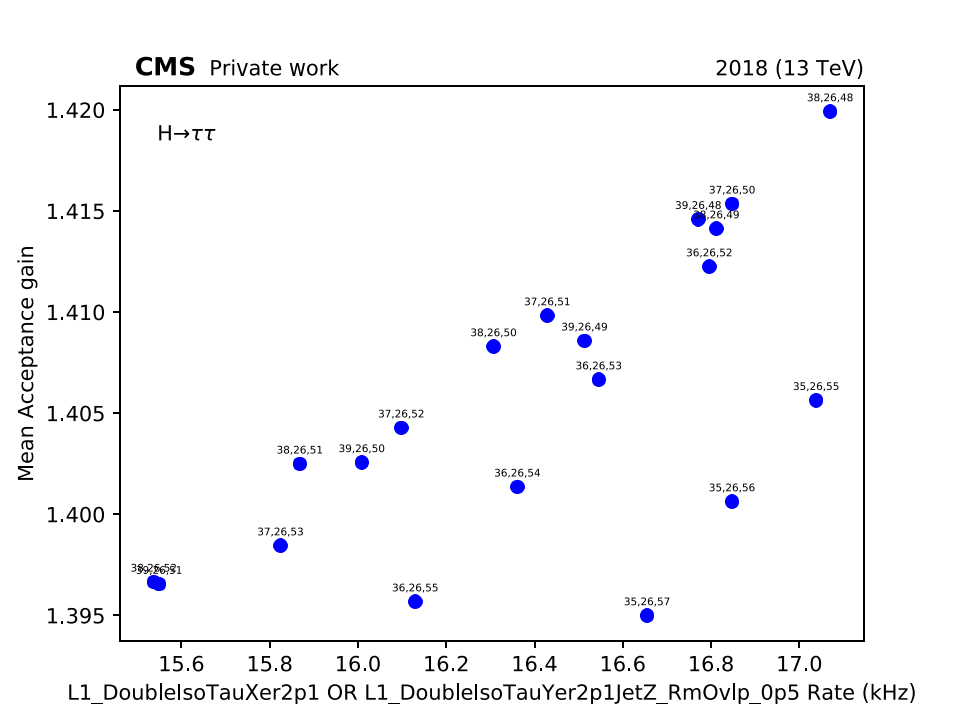
\includegraphics[width=0.49\textwidth]{Images/rate_vs_mean_acceptance__min5.0___max17.1___xx_sym__yy_sym_htt.pdf}}
\subfloat{\centering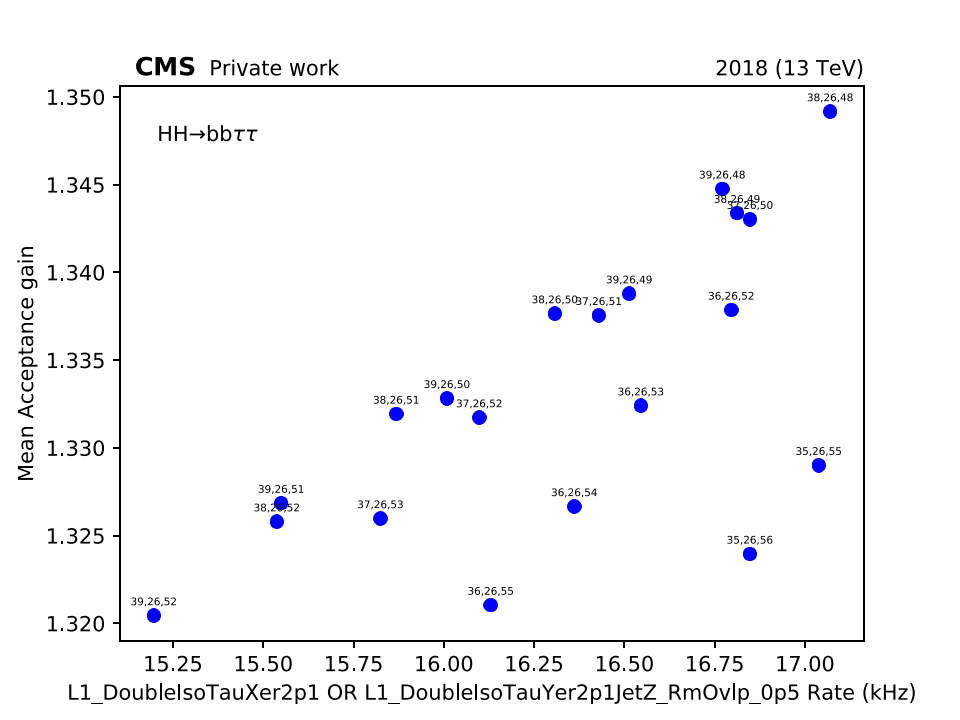
\includegraphics[width=0.49\textwidth]{Images/rate_vs_mean_acceptance__min5.0___max17.1___xx_sym__yy_sym_hhbbtt.pdf}}
\caption{Mean acceptance gain for the $H\to\tau\tau$ (left) and $HH\to bb\tau\tau$ (right) processes when considering the new trigger strategy. \textcolor{red}{(probably need to improve plots, e.g. add processes in them)}}
\label{hh:fig:l1_trig_mean_acc}
\end{figure}

\begin{table}[h!]
\begin{small}
\begin{center}
\begin{tabular}{|l|r|r|r|}
\hline
Trigger seed & \multicolumn{2}{c|}{Acceptance gain} &  Rate (kHz) \\
\hline\hline
& $H\to\tau\tau$ & $HH\to bb\tau\tau$ &  \\\hline
\texttt{L1\_DoubleIsoTau26er2p1\_Jet55\_RmOvlp\_dR0p5} & 44$\%$ & 36$\%$& $8.3 \pm 2.8$ \\
\texttt{L1\_DoubleIsoTau26er2p1\_Jet70\_RmOvlp\_dR0p5} & 34$\%$ & 29$\%$ & $5.3 \pm 1.8$ \\\hline
\end{tabular}
\end{center}
\end{small}

\caption{Rates and mean acceptance gains for the two new Double-$\tau_h$+jet seeds.}
\label{hh:tab:l1trig:allseeds}
\end{table}

%\begin{tabular}{|l|r|rr|rr|rr|r|}
%\hline
%\multicolumn{2}{|r|}{} & \multicolumn{2}{r|}{$H\to\tau\tau$, 1-jet, high $p_t$ cat.} & \multicolumn{2}{r|}{$H\to\tau\tau$, 2-jet cat.} & \multicolumn{2}{r|}{ $HH\to bb\tau\tau$} & \\\hline
% Parameters   &   Rate &    ggH &   VBFH &   ggH &  VBFH &   ggHH &   VBFHH &   Mean \\
%\hline
% 32,26,55     &  18.03 &                           1.50 &                           1.49 &                    1.35 &                    1.43 &           1.29 &           1.42 &   1.41 \\
% 32,26,70     &  16.42 &                           1.37 &                           1.38 &                    1.27 &                    1.34 &           1.25 &           1.34 &   1.33 \\
% 35,26,55     &  15.34 &                           1.47 &                           1.47 &                    1.29 &                    1.39 &           1.27 &           1.39 &   1.38 \\
% 35,26,70     &  13.27 &                           1.31 &                           1.33 &                    1.18 &                    1.27 &           1.20 &           1.28 &   1.26 \\
%\hline
%\end{tabular}


\section{Online performance of the L1 Double-$\tau_h$ + jet trigger}







\section{The HLT Double-$\tau_h$ + jet path}
\label{hh:sec:hlt_doubletaujet}

In order to trigger on Double-$\tau_h$ + jet events, an HLT path was designed and implemented, associated to the main L1 seed described in Section~\ref{hh:sec:l1seeds}. Additionally, a backup HLT path was also implemented triggered by the backup L1 seed. The structure of these path is shown in Fig.~\ref{hh:fig:hlt_path}. This structure is very similar to the existing $\tau$ paths in Run 1 and 2, but with some improvements developed for Run 3.

\begin{figure}
\begin{center}
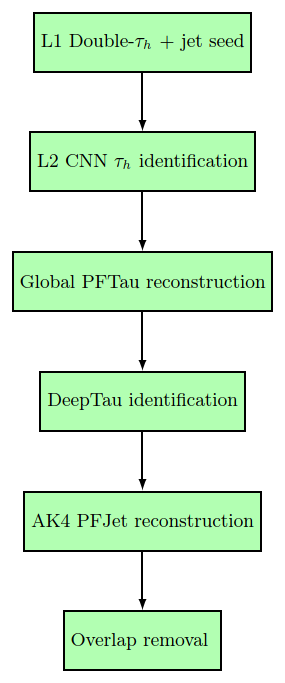
\includegraphics[width=0.4\textwidth]{Images/HLT_Path}
\end{center}
\caption{Sketch of the structure followed by the implemented HLT Double-$\tau_h$ + jet path.}
\label{hh:fig:hlt_path}
\end{figure}

For an event to pass the HLT path, the first requirement is to pass the L1 seed requirements. On top of these L1 requirements, a typical HLT di-$\tau_h$ requirement is applied \cite{intro:exp:cms_trigger}: each L1 tau is used to build a Level-2 $\tau$ by associating the L1 tau all objects that fall into a $\Delta R$ cone of 0.5 with respect to it. Then, an identification algorithm based on a Convolutional neural network (CNN) is applied, aimed to reduce the number of background objects entering the next steps of the path (more time consuming) while reducing the least possible the number of true $\tau$ filtered. This machine learning approach is one of the new additions to Run 3 $\tau$ paths, resulting in an increase of efficiency and a decrease of rate with respect to the approaches used in the previous data-taking periods. 

After building the L2 $\tau$, global PF $\tau$ are reconstructed, similarly as how it was shown in Section~\ref{intro:subsec:taus}. Another improvement with respect to Run 3 is the use of the same \deeptau algorithm as in offline reconstruction level but at HLT level, resulting in better signal purity and rate reduction.

At each step, at least a pair of $\tau$ leptons needs to survive the selection. Also, the final selected $\tau$ need to match the L1 $\tau$ used for triggering at L1 within a $\delta R$ of 0.5, and their $p_t$ must be higher than 30~GeV.

After selecting the $\tau$, the PF algorithm is used again to reconstruct the PF jets in the event. These PF jets will be selected if they satisfy an overlap removal criteria similar to the one used at L1: no matching (within a $\delta R$ of 0.5) between the jet and a pair of PF $\tau$ that passed the whole HLT selection. On top of this criteria, the jet must match a L1 jet used for triggering and have a $p_t$ higher than a given threshold. For the main HLT path (triggered with the L1 seed with the 55~GeV $p_T$ threshold), this threshold is set to 60 GeV, while for the backup path, it's set to 75 GeV.

\section{Performance of the Double-$\tau_h$ + jet HLT path}

\textcolor{red}{Shall we study as well the performance of the backup seed?}

\subsection{Expected rate using 2018 data}

To compute the rate expected from the addition of the new path, a similar approach than the one used in Section~\ref{hh:sec:l1seeds} is considered: the rate is estimated from a zero bias data sample taken during several 2018 runs but with Run-3 conditions applied (PU linearly scaled to 53 and 2748 colliding bunches). The rate obtained for this path is around 15.53 Hz. Note that, as the expected rate by an HLT path is very small (around two to three orders of magnitude smaller than the correspondent L1 seed), a lot of zero bias events are needed to obtain a reasonably accurate result. In fact, even with all the 2018 runs that were used to obtain this value, only 15 events were able to pass the trigger, so the statistical uncertainty drives the result obtained.

For the sake of validating the result, the rate was obtained in the same sample also for the main L1 seed described in Section~\ref{hh:sec:l1seeds}, resulting in a rate of 8.94~kHz, in agreement with the value obtained in that Section. 

\subsection{L1$\times$HLT efficiency}

\textcolor{red}{The definition of efficiency, the monitoring L1 paths, etc, will be included in the L1 performance section}

In order for a trigger path to be used in the analysis, the L1$\times$HLT efficiency has to be computed for both data and simulated events, so the latter can be reweighted by applying adequate scale factors. The procedure to obtain this efficiency is similar to the one shown for the L1 seeds: assuming the tau and jet legs are uncorrelated, the total efficiency can be computed as the product of the efficiency of selecting the leading $\tau$, the subleading $\tau$ and the jet.

\subsubsection{L1$\times$HLT efficiency for the tau legs}

The efficiency on the $\tau_h$ legs can be measured through a tag-and-probe technique, as was done to compute the L1 efficiency, by selecting events that were triggered by a single-muon HLT path. Among these events, the efficiency will be measured from the ones that also passed a HLT cross-trigger that requires a muon (used as tag) and an tau (used as probe). This path was implemented so that the selections applied on the muon are the same as in the single-muon path and the ones applied on the $\tau_h$ are the same requirements applied to the $\tau_h$ in the double-$\tau_h$ + jet path. The efficiency on each $\tau$ leg will be considered as independent from the other.


\subsubsection{L1$\times$HLT efficiency for the jet leg}




%\bibliographystyle{plain}
%\bibliography{../biblio.bib}





\end{document}

